\section{Results}

\subsection{Descriptive Statistics}

Environmental conditions varied substantially across the 78-day monitoring period at Spring Canyon and UDMH during the 2023-2024 overwintering season. The dataset comprised 1,894 observations collected at 30-minute intervals during daylight hours (07:00--17:00) from November 17, 2023, to February 4, 2024, totaling 947 observation hours across 115 unique deployment-day combinations.

Wind speeds ranged from complete calm to moderately strong conditions, with maximum gusts reaching 12.4 m/s (mean = 2.2 ± 1.4 m/s, median = 2.2 m/s). The interquartile range of 1.3--3.0 m/s indicated that most observations occurred under relatively mild wind conditions. Temperature showed considerable variation throughout the monitoring period, ranging from 3.0 to 30.0°C (mean = 14.6 ± 3.8°C, median = 14.0°C), with an interquartile range of 12.5--17.0°C typical of California coastal winter conditions. Direct solar exposure occurred in 31.7\% of observations (n = 601), with butterflies actively basking when present in sunlight, averaging 17.0 individuals in direct sun (range: 1--295).

Monarch abundance exhibited high variability across sites and time periods. Butterfly counts ranged from 0 to 770 individuals per observation, with a mean of 81.4 ± 100.0 butterflies and a median of 37 butterflies. The wide interquartile range (9--119 butterflies) reflected substantial variation in cluster sizes. Zero-count observations, representing either the beginning of cluster formation or cluster dissolution, comprised 2.3\% of the dataset (n = 43).

Cluster sizes varied markedly among the 10 deployment locations. Site SC10 recorded the largest aggregation with 770 monarchs, while mean abundances ranged from 0 at SC9 to 325.8 at UDMH2. Eight deployments observed maximum cluster sizes exceeding 100 butterflies, with mean maximum cluster size across sites reaching 315.6 individuals. This variation in cluster sizes across deployments reflects the heterogeneous distribution of monarchs across overwintering microhabitats within the study sites.

The comprehensive temporal coverage, with observations at 30-minute intervals capturing 16.5 observations per deployment-day on average, provided fine-scale resolution of monarch behavioral responses to changing environmental conditions. Peak observation activity occurred at 16:00 hours (196 observations), corresponding with afternoon warming periods when monarchs typically exhibit increased movement.

\subsection{Summary of Data and Model Selection}

Environmental factors drove monarch abundance changes in 1,894 paired observations from 115 monitoring periods at two overwintering sites during the 2023–2024 season. After expanding the candidate set to include tensor–product interactions (ti), testing of 52 candidate models identified model M50 as the best‑fit.

Model M50 included smooth terms for previous butterfly count, temperature, and time since sunrise, plus a tensor–product interaction between maximum wind speed and butterflies in direct sun. The AIC comparison favored M50 (AIC ≈ 8078.0) over the next best models (ΔAIC ≥ 3.8). We report full model selection details via the exported table.

\begin{table}[htbp]
\centering
\caption{Top five candidate models ranked by AIC for the 30‑minute analysis.}
\label{tab:model_selection}
\begin{table}

\caption{\label{tab:export-model-selection-table}Top 5 candidate models ranked by AIC for monarch butterfly abundance change analysis. All terms are smooth unless marked as (linear). Wind p-value shows significance of max_gust term when present in model.}
\centering
\begin{tabular}[t]{llrrrrl}
\toprule
Model ID & Model Terms & AIC & <U+0394>AIC & AIC Weight & df & Wind p-value\\
\midrule
M50 & \textbullet\ Previous butterfly count\\ \textbullet\ Temperature\\ \textbullet\ Time since sunrise\\ \textbullet\ ti(Maximum wind speed, Butterflies in direct sun) & 8078.029 & 0.000 & 0.8559 & 15 & 5.55e-05\\
M23 & \textbullet\ Previous butterfly count\\ \textbullet\ Temperature\\ \textbullet\ Butterflies in direct sun\\ \textbullet\ Time since sunrise & 8081.848 & 3.820 & 0.1268 & 14 & NA\\
M22 & \textbullet\ Previous butterfly count\\ \textbullet\ Temperature (linear)\\ \textbullet\ Butterflies in direct sun\\ \textbullet\ Time since sunrise & 8086.644 & 8.615 & 0.0115 & 13 & NA\\
M24 & \textbullet\ Previous butterfly count\\ \textbullet\ Maximum wind speed\\ \textbullet\ Temperature\\ \textbullet\ Butterflies in direct sun\\ \textbullet\ Time since sunrise & 8088.049 & 10.020 & 0.0057 & 16 & 0.218\\
M52 & \textbullet\ Temperature\\ \textbullet\ Time since sunrise\\ \textbullet\ ti(Maximum wind speed, Butterflies in direct sun) & 8096.722 & 18.693 & 0.0001 & 13 & 1.13e-05\\
\bottomrule
\end{tabular}
\end{table}

\end{table}

\subsection{Analysis of the Best-Fit Model}

The best‑fit model (M50) included three smooth main effects and one tensor–product interaction:

\begin{equation}
\text{Change in abundance} \sim s(\text{Previous butterfly count}) + s(\text{Temperature}) + s(\text{Time since sunrise}) + ti(\text{Maximum wind speed},\, \text{Butterflies in direct sun}).
\end{equation}

All three smooth main effects were significant, and the wind × sun interaction was strongly supported in the AIC comparison (Table~\ref{tab:model_selection}). Smooth‑term statistics for the best model are provided via the exported table.

\begin{table}[htbp]
\centering
\caption{Summary of smooth terms in the best‑fit model (M50). EDF represents effective degrees of freedom.}\label{tab:smooth_terms}
\begin{table}

\caption{Summary of smooth terms in the best-fit GAM model}
\centering
\begin{tabular}[t]{llrrrl}
\toprule
  & Smooth Term & EDF & Ref. df & F & p-value\\
\midrule
s(total\_butterflies\_t\_lag) & Lagged roost size & 2.621 & 2.621 & 12.020 & 8.26e-07\\
s(temperature\_avg) & Average temperature & 3.930 & 3.930 & 3.230 & 0.0283\\
s(butterflies\_direct\_sun\_t\_lag) & Direct sun exposure & 1.534 & 1.534 & 19.356 & 1.22e-05\\
s(time\_within\_day\_t) & Time within day & 4.898 & 4.898 & 8.901 & < 2e-16\\
\bottomrule
\end{tabular}
\end{table}

\end{table}

Partial effects for the three smooth main effects are shown in Figure~\ref{fig:partial_effects}. The previous butterfly count showed a non‑linear negative relationship consistent with proportionally greater departures from larger aggregations. Time since sunrise captured a diurnal pattern with morning departures and afternoon returns. Temperature displayed a non‑linear response with minimal effects below the 12.7–16°C flight threshold and reformation at moderate temperatures.

\begin{figure}[htbp]
\centering
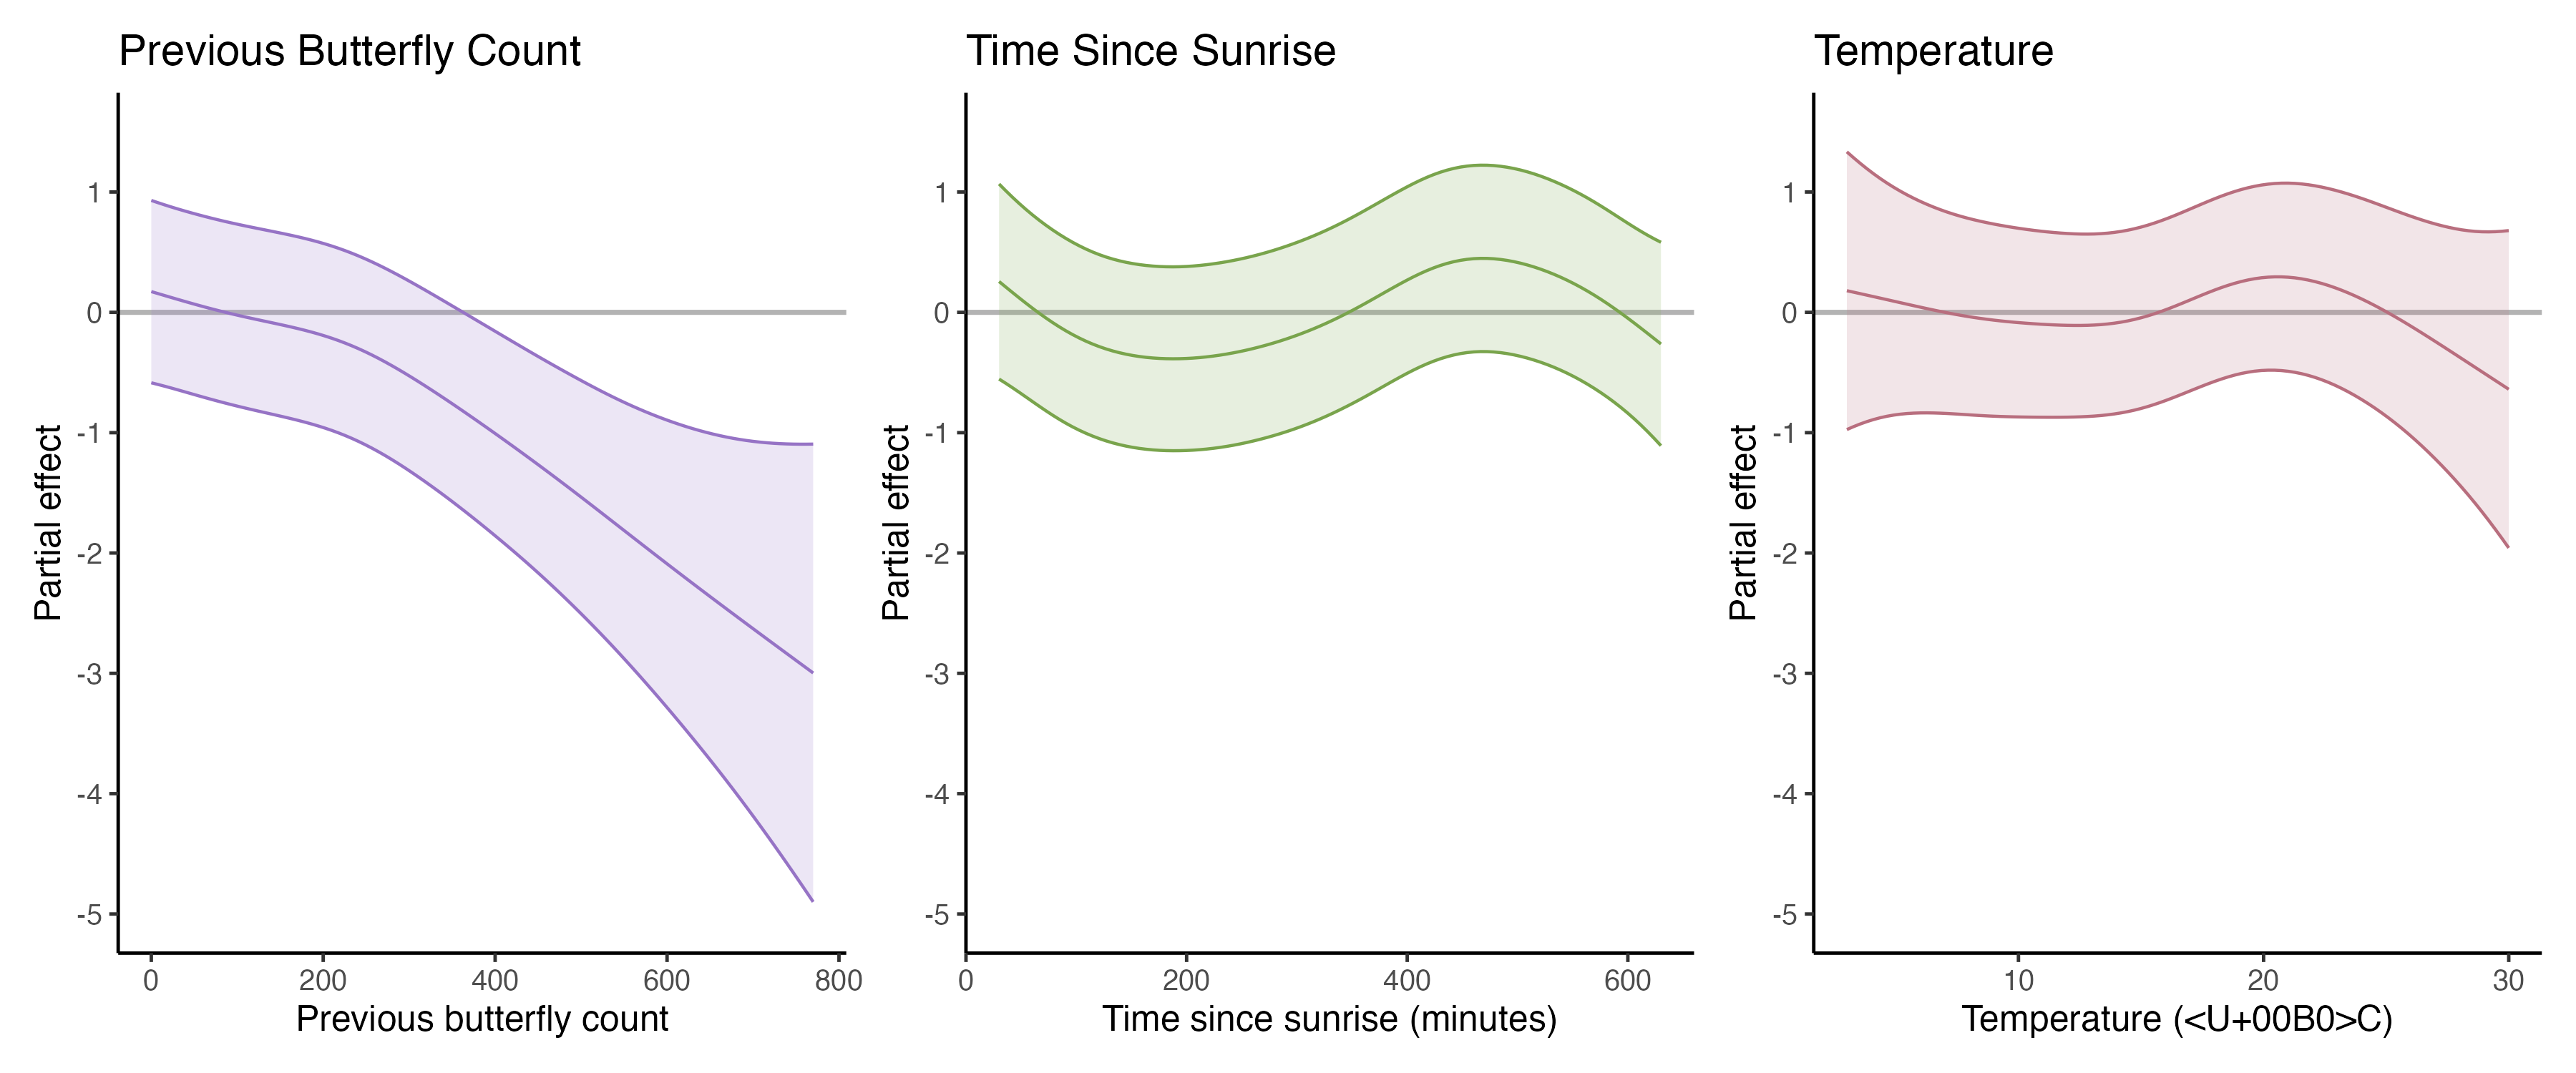
\includegraphics[width=\textwidth]{figures/results/combined_partial_effects_1x3_final.png}
\caption{Partial effects for the three smooth main effects in the best model: previous butterfly count (purple), time since sunrise (green), and temperature (mauve). Solid lines show estimated smooths with 95\% confidence intervals (shaded regions), on a shared y‑axis scale.}\label{fig:partial_effects}
\end{figure}

\subsection{Evaluation of the Disruptive Wind Hypothesis}

Our analysis did not support a simple disruptive wind effect or a fixed 2~m/s threshold at the 30‑minute scale. Instead, when wind was selected it entered as a smooth interaction with direct sun exposure (ti), indicating that any wind association with departures is conditional on solar exposure rather than monotonic or threshold‑based. A sensitivity analysis using ‘minutes above 2~m/s’ performed poorly and did not rank among top candidates (Table~\ref{tab:threshold_model_selection}). Visually, the relationship between wind and abundance change shows no disruption at the 2~m/s boundary (Figure~\ref{fig:wind_scatter}).

\begin{table}[htbp]
\centering
\caption{Model selection results from sensitivity analysis using wind threshold predictor (minutes with wind speed > 2 m/s). Poor model performance (high $\Delta$AIC values) demonstrates lack of support for the 2 m/s disruption threshold.}
\label{tab:threshold_model_selection}
\begin{tabular}{lllrrr}
\hline
Model & Terms & AIC & $\Delta$AIC & Weight & Wind p \\
\hline
T24 & Previous butterfly count, Minutes above 2~m/s, & 8089.4 & 7.6 & 0.021 & 0.372 \\
    & Temperature, Butterflies in direct sun, Time since sunrise & & & & \\
T44 & Minutes above 2~m/s, Temperature, & 8108.4 & 26.5 & <0.001 & 0.256 \\
    & Butterflies in direct sun, Time since sunrise & & & & \\
T21 & Previous butterfly count, Minutes above 2~m/s, & 8110.6 & 28.7 & <0.001 & 0.053 \\
    & Temperature, Butterflies in direct sun & & & & \\
T43 & Minutes above 2~m/s, Temperature (linear), & 8115.5 & 33.7 & <0.001 & 0.275 \\
    & Butterflies in direct sun, Time since sunrise & & & & \\
T19 & Previous butterfly count, Minutes above 2~m/s, & 8119.8 & 37.9 & <0.001 & 0.078 \\
    & Temperature (linear), Butterflies in direct sun & & & & \\
\hline
\end{tabular}
\end{table}

Third, wind's effects did not scale with intensity. The relationship remained flat across all observed wind speeds (0–12~m/s), with confidence intervals consistently encompassing zero (Figure~\ref{fig:wind_scatter}).

\begin{figure}[htbp]
\centering
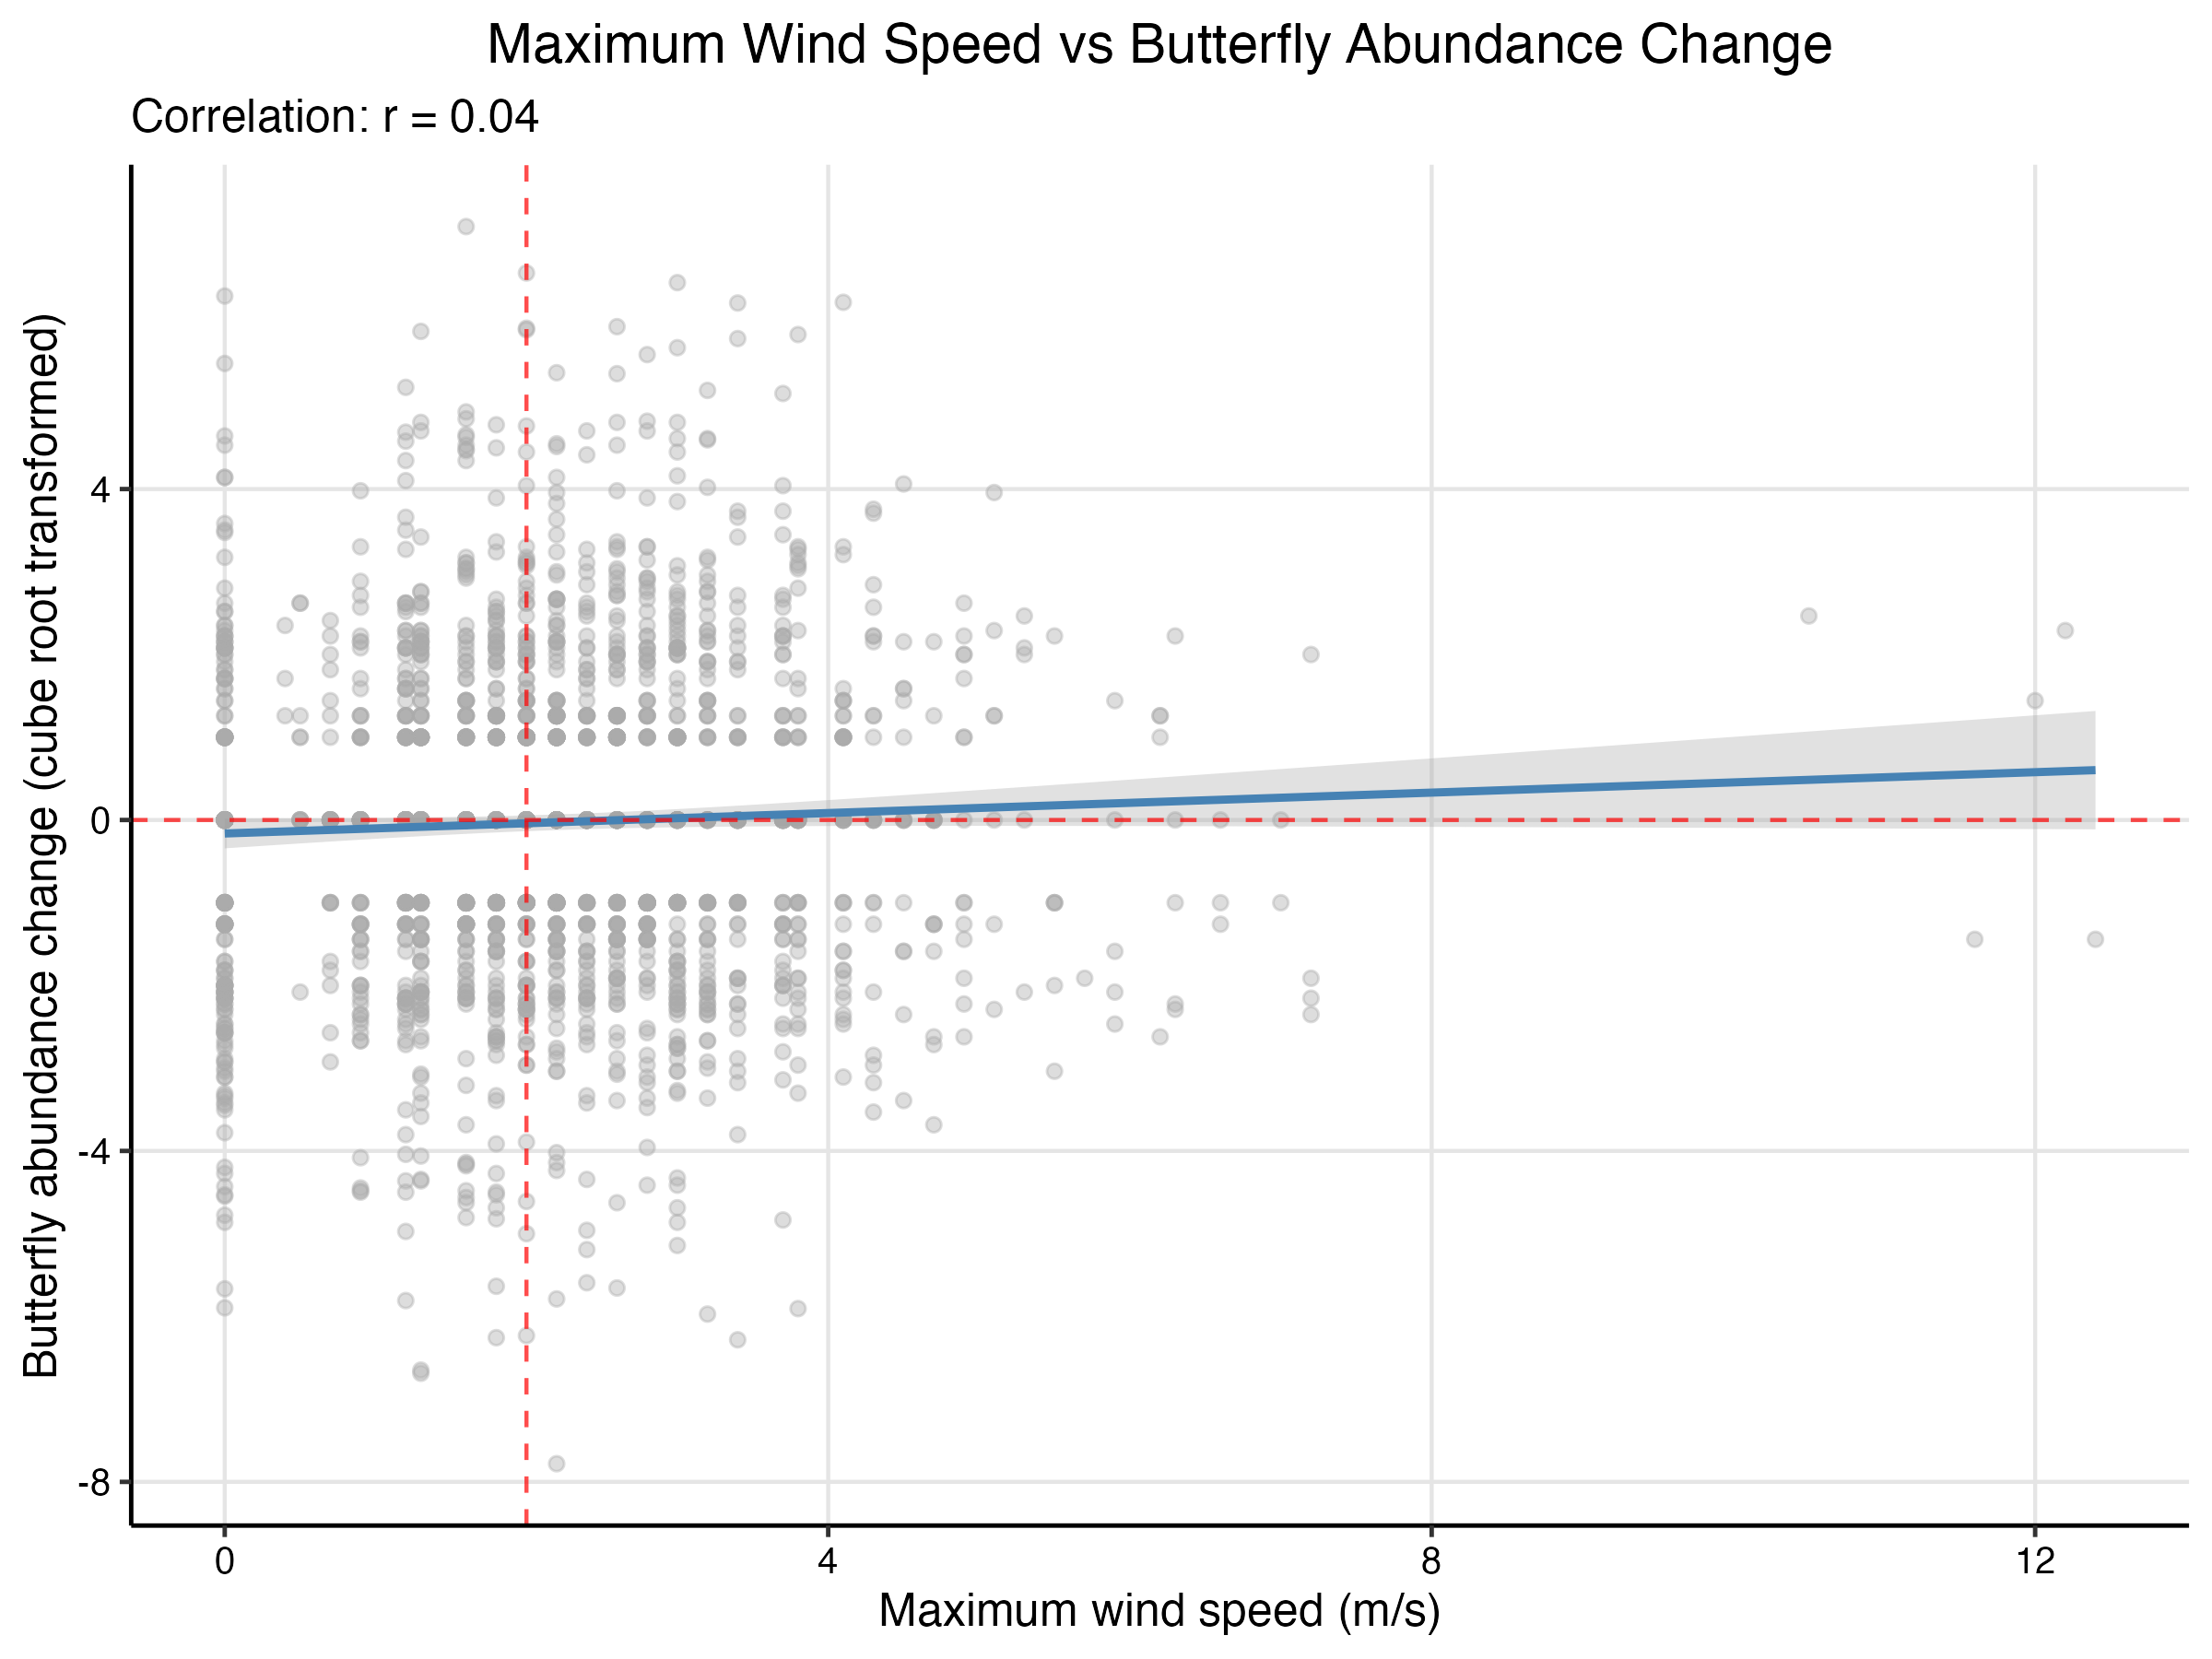
\includegraphics[width=0.8\textwidth]{figures/results/wind_hypothesis_scatter.png}
\caption{Relationship between maximum wind speed (m/s) and monarch abundance change. The red dashed line shows the proposed 2 m/s disruptive wind threshold, while the flat trend line indicates no effect of wind on butterfly departures. Points represent 30-minute observation periods.}\label{fig:wind_scatter}
\end{figure}

\subsection{Statistical Power to Detect Wind Effects}

Post-hoc power analysis confirmed our study had adequate statistical power to detect biologically meaningful wind effects (Table~\ref{tab:power_analysis}). With 1,894 paired observations, we achieved 87.5\% power to detect moderate effect sizes (0.15 standard deviations) and 98.5\% power to detect larger effects (0.20 standard deviations). Power for small effects (0.10 standard deviations) was 56\%, while very small effects (0.05 standard deviations) yielded only 16.5\% power. These results indicate that our failure to detect wind effects is unlikely due to insufficient statistical power for effect sizes of biological relevance.

\begin{table}[htbp]
\centering
\caption[Statistical power to detect wind effects]{Estimated power to detect wind effects of varying magnitudes. Effect sizes are expressed in standard deviations of the response variable (cube root transformed change in butterfly abundance).}
\label{tab:power_analysis}
\begin{tabular}[t]{lrrl}
\toprule
  & Effect Size (SD units) & Power (Proportion) & Power (\%)\\
\midrule
0.05 & 0.05 & 0.165 & 16.5\%\\
0.1 & 0.10 & 0.560 & 56\%\\
0.15 & 0.15 & 0.875 & 87.5\%\\
0.2 & 0.20 & 0.985 & 98.5\%\\
\bottomrule
\end{tabular}
\end{table}


\subsection{Dynamic Window Analysis}

To test whether cumulative weather exposure influenced day-to-day roost dynamics, we analyzed 96 consecutive-day pairs from the same deployment dataset using biologically-aligned temporal windows. The primary analysis employed a sunset window spanning from the previous day's maximum count to the current day's last observation (mean duration = 29.6 hours), capturing the full period from peak aggregation through the subsequent roosting decision. A secondary analysis using fixed 24-hour windows (n = 94 pairs) provided a sensitivity test of our findings.

Daily maximum cluster sizes ranged from 0 to 770 butterflies (mean = 134.7 ± 138.1), with day-to-day changes in maximum count ranging from losses of 376 butterflies to gains of 464 butterflies (mean change = -10.5 ± 111.6). Within the sunset windows, maximum wind gusts ranged from 2.0 to 12.8 m/s (mean = 4.5 ± 1.8 m/s), with all observation windows exceeding the proposed 2 m/s threshold. Cumulative direct sun exposure varied from 0 to 1,122 butterfly-observations in sunlight per window (mean = 139.8 ± 206.9), reflecting diverse thermal exposure conditions across monitoring days.

\subsubsection{Model Selection}

Among 76 candidate models tested, the sunset window analysis identified a smooth interaction between maximum wind gust and cumulative direct sun exposure as the best-supported structure (Table~\ref{tab:dynamic_model_selection}). This model achieved an adjusted R² of 0.397, with the interaction term showing strong statistical support (edf = 6.68, F = 4.10, p < 0.001). The 24-hour window sensitivity analysis converged on the same interaction structure, though with reduced explanatory power (adjusted R² = 0.232) and weaker statistical significance (edf = 3.54, F = 3.59, p = 0.020), confirming the robustness of the finding across window definitions.

\begin{table}[htbp]
\centering
\caption{Top five models from dynamic window analyses ranked by AICc. The sunset window represents the primary biologically-aligned analysis (n = 96), while the 24-hour window provides a sensitivity test (n = 94). Convergence on wind-sun interaction models across both approaches supports conditional rather than threshold-based wind effects.}
\label{tab:dynamic_model_selection}
\begin{tabular}{lrrr}
\hline
Model Terms & AICc & $\Delta$AICc & Weight \\
\hline
\multicolumn{4}{l}{\textit{Sunset Window Analysis}} \\
Baseline + ti(wind\_gust, sun\_exposure) & 351.2 & 0.0 & 0.312 \\
Baseline + wind\_gust $\times$ sun\_exposure & 352.8 & 1.6 & 0.141 \\
Baseline + te(wind\_gust, sun\_exposure) & 353.1 & 1.9 & 0.121 \\
Baseline + s(wind\_gust) + s(sun\_exposure) & 355.4 & 4.2 & 0.038 \\
Baseline controls only & 356.7 & 5.5 & 0.020 \\
\\
\multicolumn{4}{l}{\textit{24-Hour Window Sensitivity Analysis}} \\
Baseline + ti(wind\_gust, sun\_exposure) & 367.5 & 0.0 & 0.298 \\
Baseline + wind\_gust $\times$ sun\_exposure & 368.9 & 1.4 & 0.148 \\
Baseline + s(wind\_gust) + s(sun\_exposure) & 369.3 & 1.8 & 0.121 \\
Baseline + te(wind\_gust, sun\_exposure) & 370.1 & 2.6 & 0.081 \\
Baseline controls only & 372.4 & 4.9 & 0.026 \\
\hline
\end{tabular}
\end{table}

\subsubsection{Interaction Pattern}

The partial effect surfaces revealed consistent patterns across both analyses (Figure~\ref{fig:dynamic_interaction}). Positive effects on daily roost change, indicating aggregation gains, concentrated at moderate sun exposure (500-1,500 butterfly-observations) combined with moderate wind speeds (5-10 m/s). At low sun exposure (<200 butterfly-observations), the partial effects remained near zero across all wind speeds. At very high sun exposure (>2,000 butterfly-observations), effects became negative regardless of wind conditions. The surface showed no evidence of disruption at the proposed 2 m/s threshold, with the gradient remaining continuous across this boundary.

\begin{figure}[htbp]
\centering
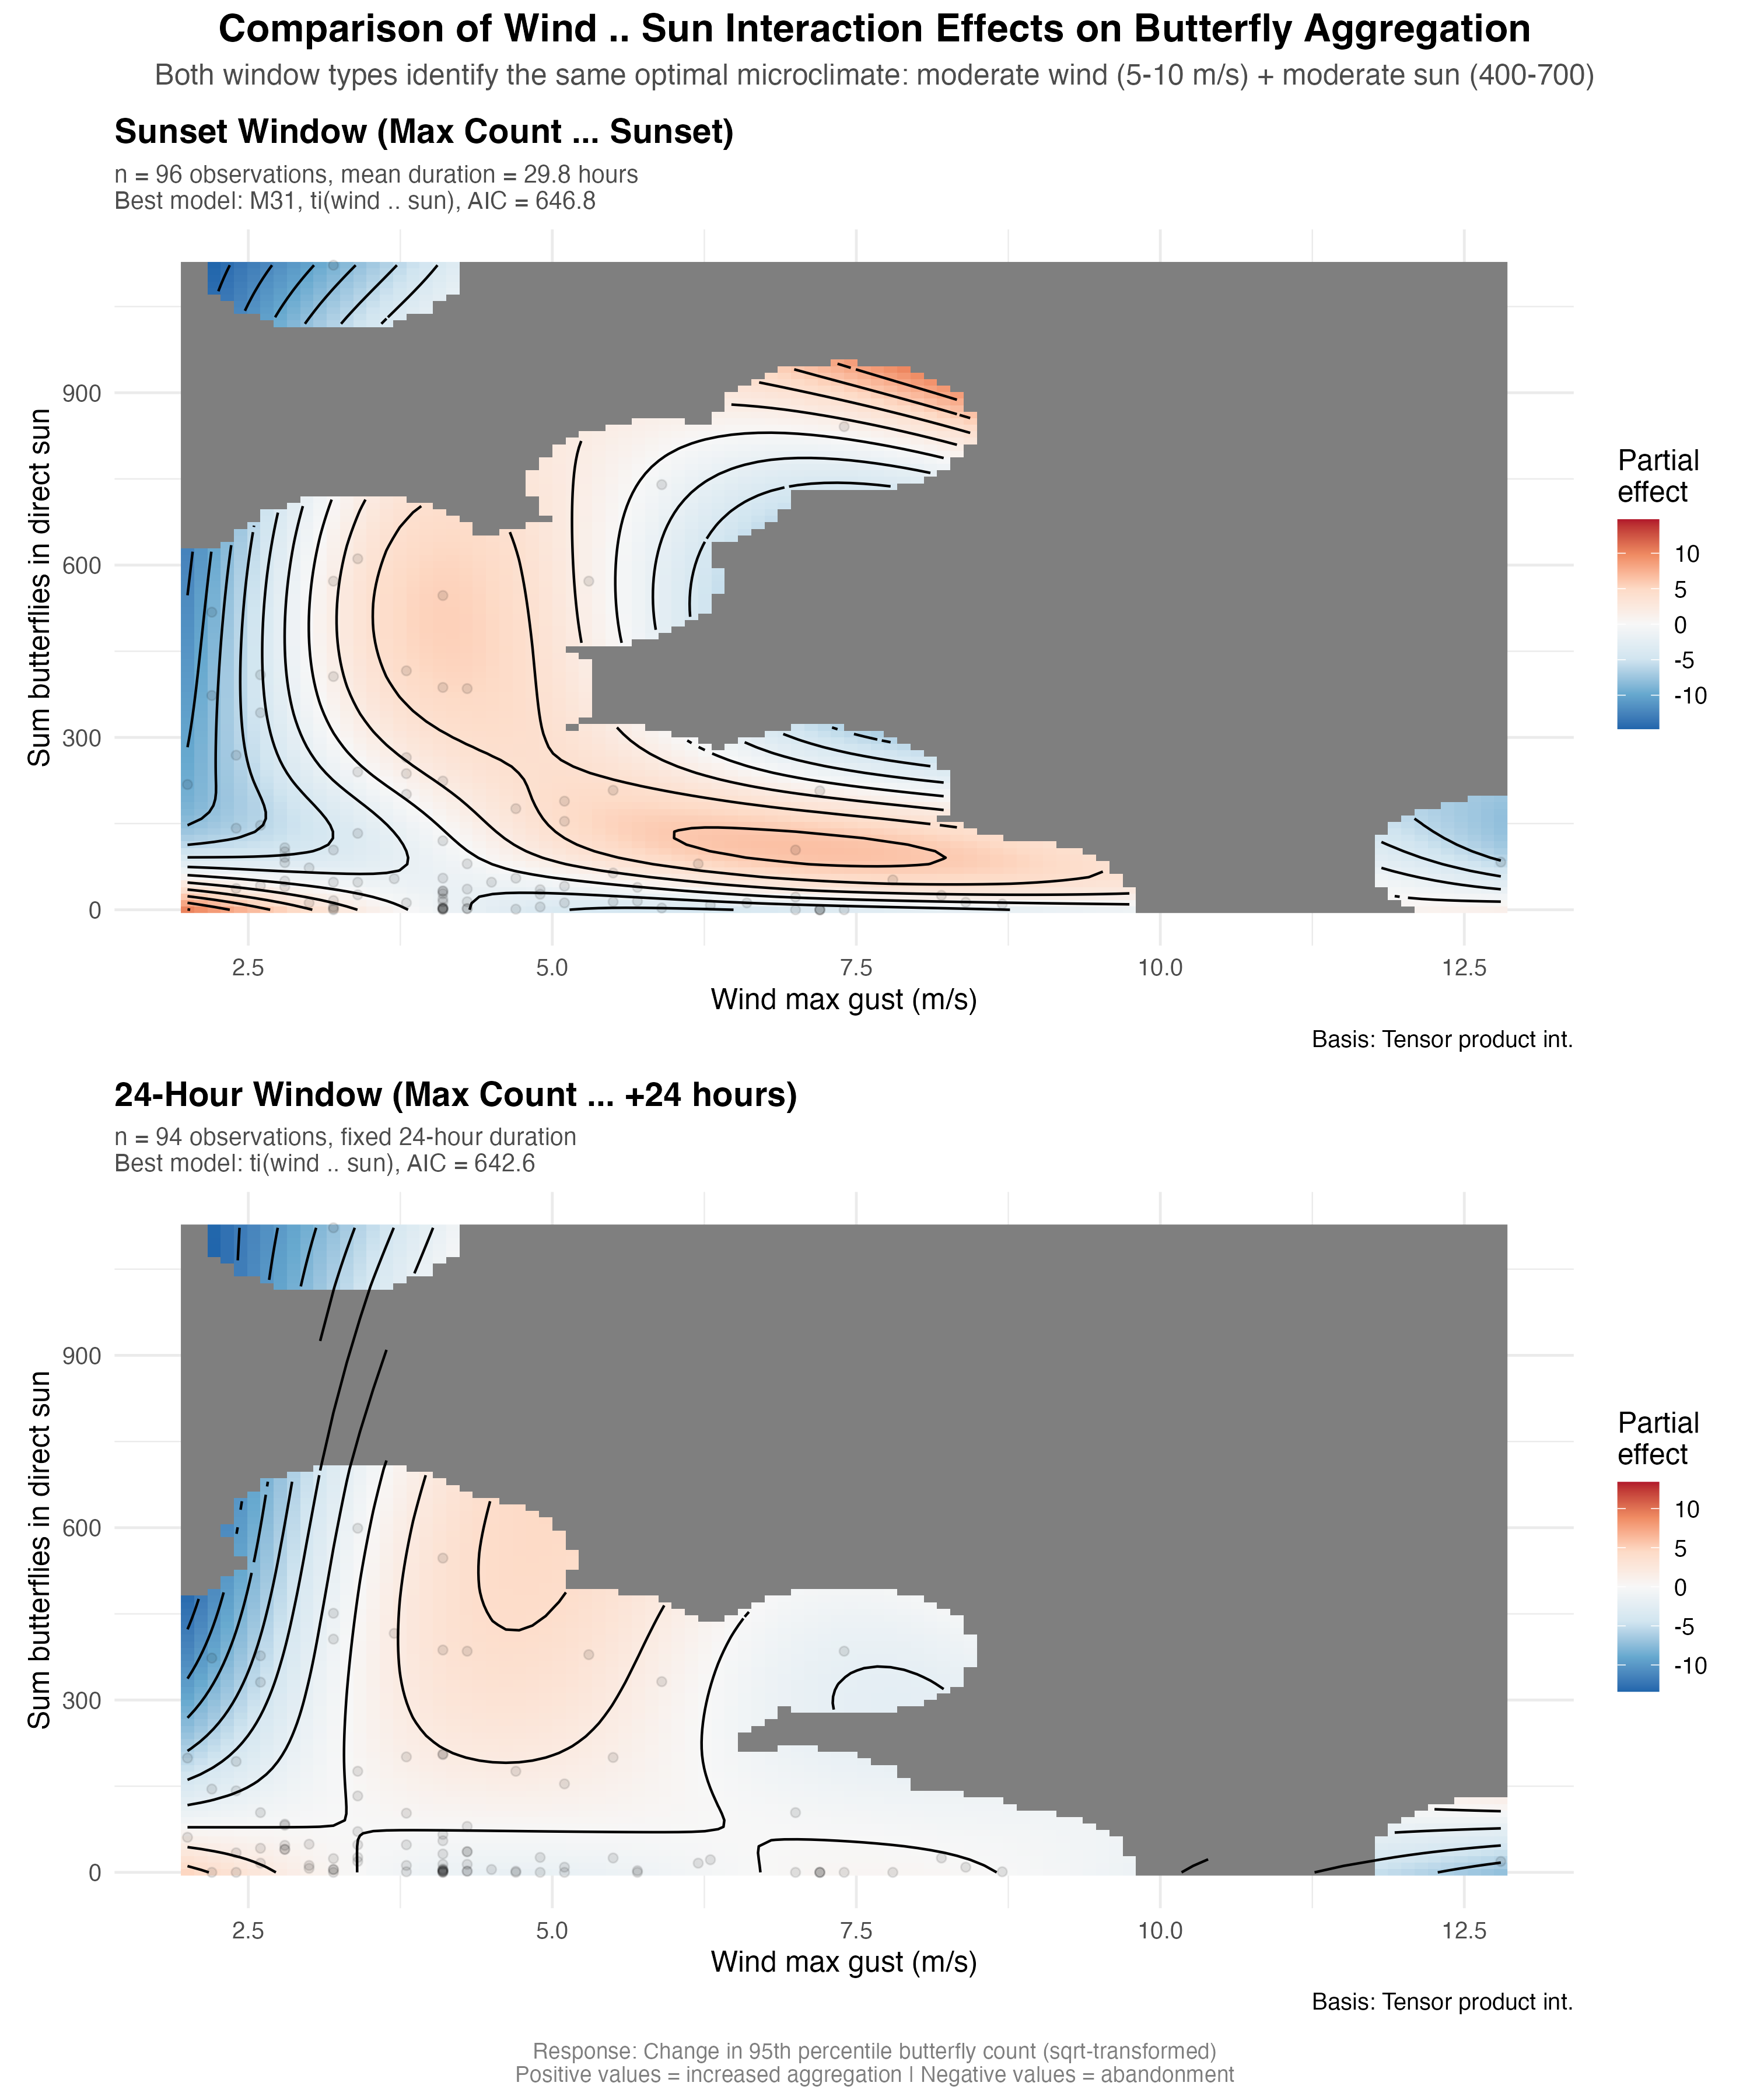
\includegraphics[width=\textwidth]{figures/results/window_comparison_interaction.png}
\caption{Partial effect surfaces from the best-fit generalized additive mixed models showing the interaction between maximum wind gust and cumulative direct sun exposure on daily roost change. Positive values (red) indicate aggregation gains; negative values (blue) indicate losses. Gray regions denote parameter combinations without data support. The sunset window analysis (left) shows the primary result, with the 24-hour window (right) providing sensitivity confirmation.}
\label{fig:dynamic_interaction}
\end{figure}

No models incorporating the 2 m/s threshold as a discrete predictor ranked among the top candidates in either analysis. Models testing minutes above 2 m/s, cumulative gust exposure above 2 m/s, or binary threshold indicators consistently performed worse than models with continuous wind-sun interactions ($\Delta$AICc > 10 for all threshold models).

\subsection{Model Diagnostics}

Model residuals showed distinct linear banding patterns consistent with the discrete counting method used to estimate butterfly abundance, while the Q-Q plot indicated approximately normal residual distribution with minor tail deviations (Figure~\ref{fig:diagnostics}).

\begin{figure}[htbp]
\centering
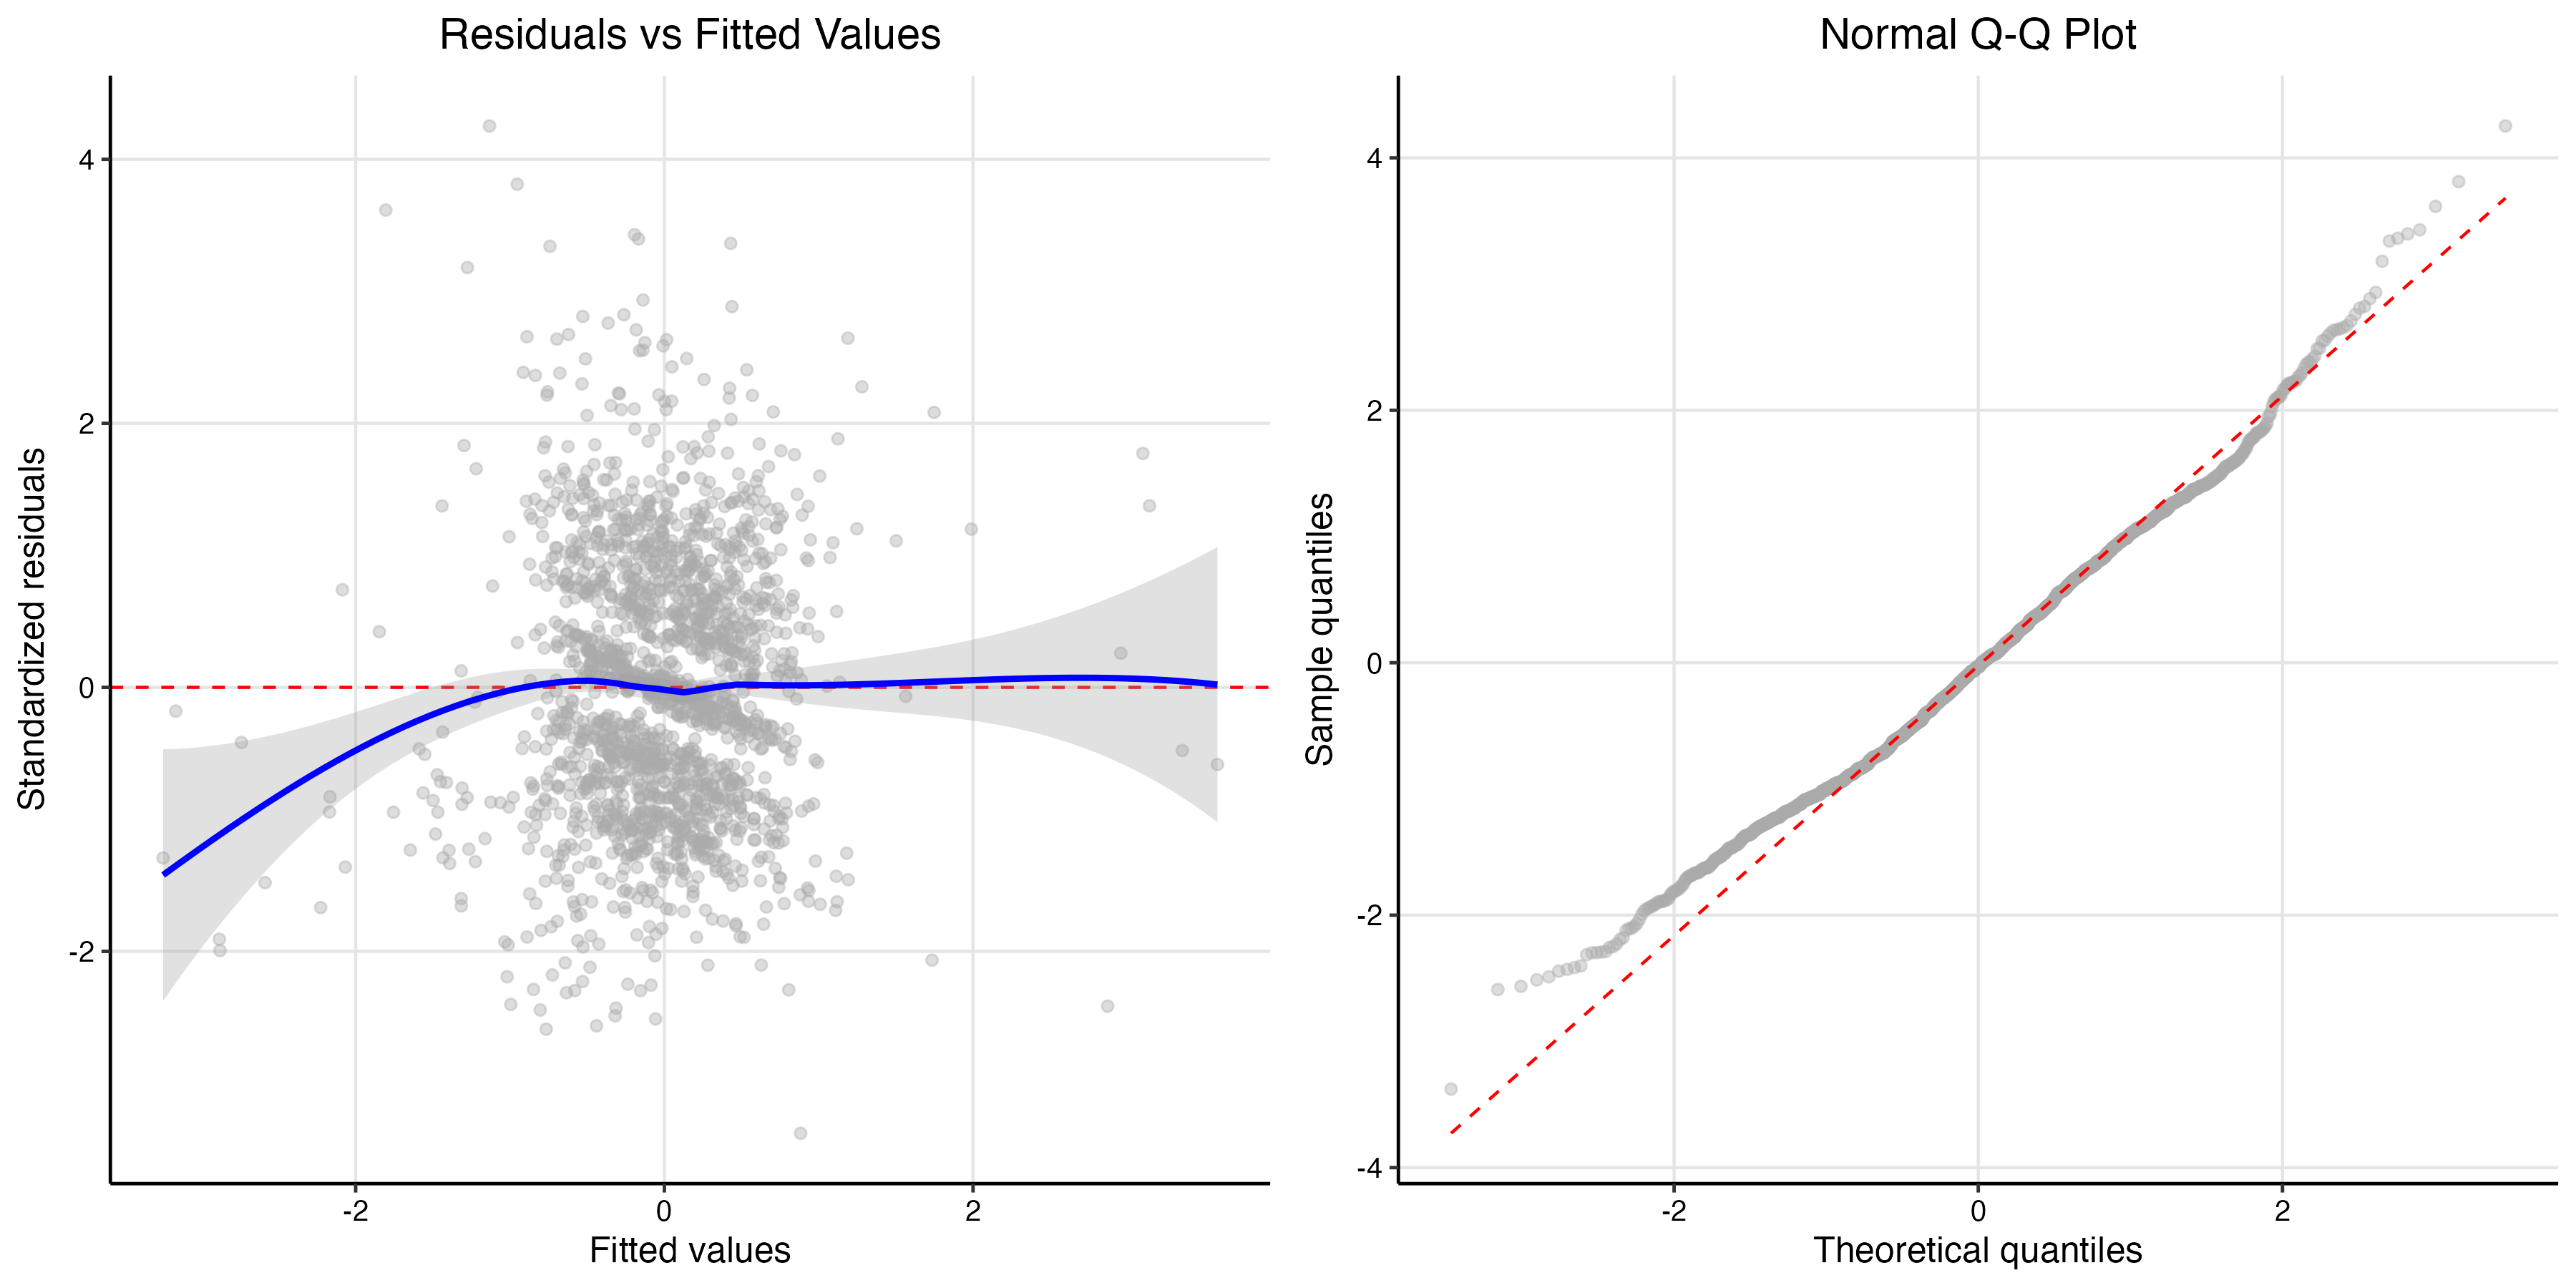
\includegraphics[width=\textwidth]{figures/results/combined_diagnostics.png}
\caption{Model diagnostics for the best model. Left: Residuals versus fitted values showing banding consistent with discrete counting; right: Normal Q-Q plot of residuals showing reasonable normality with minor tail deviations.}\label{fig:diagnostics}
\end{figure}

% To update figures, rerun the quarto doc masters-analysis/analysis/monarch_gam_analysis.qmd (separate repo) and copy the thesis-exports folder to this one.
